\documentclass[12pt]{article}
\usepackage{tikz}

% global styles
\tikzset{help lines/.style={color=gray!50,very thin,step=.5}}

\begin{document}
First tikz picture.

\begin{center}
  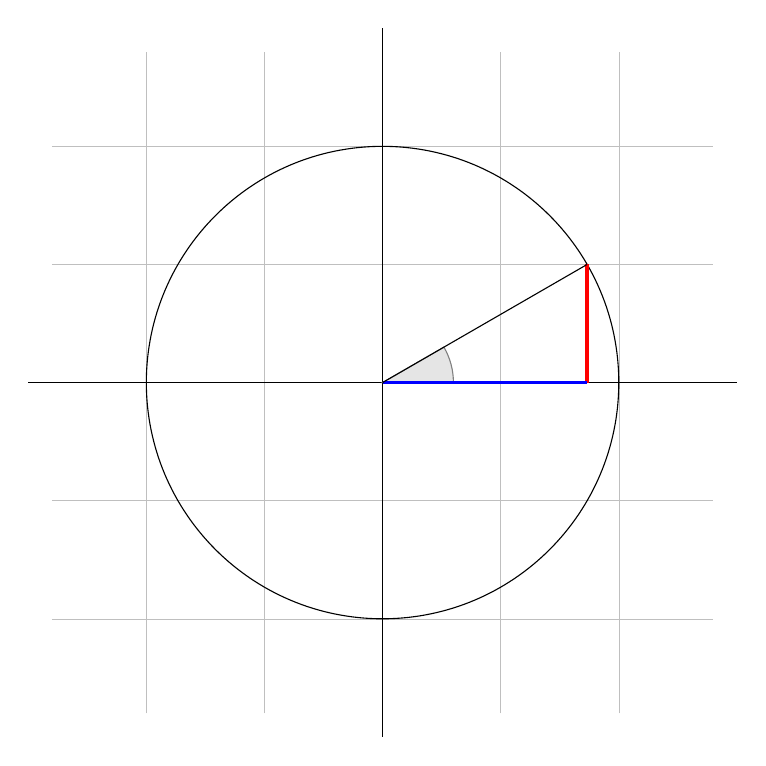
\begin{tikzpicture}[scale=3]
    \draw[help lines] (-1.4,-1.4) grid (1.4,1.4);
    \draw (-1.5,0) -- (1.5,0);
    \draw (0,-1.5) -- (0,1.5);
    \draw (0,0) circle [radius=1cm];
    \filldraw[fill=gray!20,draw=black!50] (0,0) -- (3mm,0) arc [start angle=0, end angle=30, radius=3mm] -- cycle;
    \draw[red, very thick] (30:1cm) -- +(0,-0.5);
    \draw[blue, very thick] (30:1cm) +(0,-0.5) -- (0,0);
    \draw (0,0) -- (30:1cm);
  \end{tikzpicture}
\end{center}
\end{document}
